\documentclass[a4paper,11pt]{scrreprt}
%==================================================
% Pakete
%==================================================
\usepackage[T1]{fontenc}
\usepackage[utf8]{inputenc}
\usepackage[ngerman]{babel}
\usepackage{lmodern}
\usepackage[a4paper,left=2.5cm,right=2.5cm,top=2.5cm,bottom=2.5cm]{geometry}
\usepackage{amsmath,amssymb,amsfonts,mathtools}
\usepackage{graphicx}
\usepackage{float}
\usepackage{booktabs}
\usepackage{array}
\usepackage{enumitem}
\usepackage{xcolor}
\usepackage[most]{tcolorbox}
\usepackage{tikz}
\usetikzlibrary{positioning,arrows.meta,calc}
\usepackage{siunitx}
\usepackage{caption}
\usepackage[hidelinks]{hyperref}
\usepackage[ngerman]{cleveref} % zuletzt laden

\graphicspath{{abbildungen/}{Messdaten_05_11_26/}{Versuchsbilder/}}

% ---------- Farben und Boxen ----------
\definecolor{dunkelblau}{RGB}{20,50,110}
\definecolor{ergebnisgruen}{RGB}{30,110,60}
\definecolor{hinweisorange}{RGB}{190,100,10}

\newtcolorbox{aufgabe}[1]{
  enhanced, breakable, colback=dunkelblau!4, colframe=dunkelblau,
  fonttitle=\bfseries, title={#1}, arc=1.5mm
}
\newtcolorbox{ergebnis}[1][Ergebnis]{
  enhanced, breakable, colback=ergebnisgruen!6, colframe=ergebnisgruen,
  fonttitle=\bfseries, title={#1}, arc=1.5mm
}
\newtcolorbox{hinweis}[1][Hinweis]{
  enhanced, breakable, colback=hinweisorange!6, colframe=hinweisorange,
  fonttitle=\bfseries, title={#1}, arc=1.5mm
}

\newcommand{\ue}{\ddot{u}}

\sisetup{
  output-decimal-marker = {,},
  per-mode = symbol,
  inter-unit-product = \ensuremath{{}\cdot{}}
}
\renewcommand{\arraystretch}{1.3}
\bibliographystyle{unsrt}

%==================================================
\begin{document}

\title{2.~Versuchsprotokoll zum Versuch~2 -- Drehstromtransformator\\[0.5em]
  \large Protokoll für das Labor Elektrische Maschinen an der Ostfalia Hochschule, WiSe 2026/27}
\author{Gruppe DoB 5\\[0.5em]
  Felix Sebastian Mayer [EITiP] (Matrikelnr.~70492245)\\
  Hsen Zayati [EIT] (Matrikelnr.~70515042)}
\date{Versuchsdatum: 5.~November 2026\\[0.3em] Abgabe: \today}
\maketitle

\tableofcontents

%==================================================
\chapter{Einleitung}

Im zweiten Versuch der fünfteiligen Versuchsreihe wird ein Drehstromtransformator untersucht. Transformatoren sind die Grundlage der Energieübertragung: Sie setzen die Spannung zwischen Erzeugung, Übertragung und Verbraucher um und arbeiten dabei mit Wirkungsgraden von deutlich über \SI{95}{\percent}. Aus wenigen Messungen lassen sich die Elemente des Ersatzschaltbilds und damit das gesamte Betriebsverhalten bestimmen.

Der Versuch gliedert sich in folgende Teile:
\begin{enumerate}[nosep]
  \item \textbf{Leerlaufversuch:} Die Primärseite wird bei offener Sekundärseite mit veränderlicher Spannung gespeist. Daraus folgen der Magnetisierungsstrom, die Eisenverluste sowie die Querelemente $R_\mathrm{Fe}$ und $X_\mathrm{h}$ des Ersatzschaltbilds.
  \item \textbf{Kurzschlussversuch:} Bei kurzgeschlossener Sekundärseite wird der Strom bis etwa zum Nennstrom erhöht. Daraus folgen die Kurzschlussspannung $u_\mathrm{k}$, die Kupferverluste sowie die Längselemente $R_\mathrm{k}$ und $X_\mathrm{k}$. Gemessen wurde in den Schaltungen Yy und Yz.
  \item \textbf{Belastungsversuch:} Der Transformator (Schaltung Yz) wird ohmsch, ohmsch-induktiv und ohmsch-kapazitiv belastet. Bestimmt werden Wirkungsgrad, Spannungsänderung und Blindleistungsbedarf.
  \item \textbf{Einschaltversuch (Rush-Effekt):} Der leerlaufende Transformator wird mehrfach direkt ans Netz geschaltet und der Einschaltstrom mit dem Oszilloskop aufgezeichnet.
\end{enumerate}

%==================================================
\chapter{Versuchsvorbereitende Aufgaben}
% Versuchsvorbereitende Aufgaben (Kapitel 2)
\section{Parallelschaltung von Transformatoren}\label{sec:a1}

\begin{aufgabe}{Aufgabenstellung}
Geben Sie einige Schaltgruppenkombinationen an, die parallelgeschaltet werden können. Was ist bei der Parallelschaltung von Transformatoren darüber hinaus zu beachten?
\end{aufgabe}

\textbf{Schaltgruppenkombinationen.} Zwei Transformatoren dürfen parallelgeschaltet werden, wenn sie dieselbe Kennzahl (Uhrzeigerzahl, $\varphi = \text{Kennzahl}\cdot\SI{30}{\degree}$) besitzen, da sonst zwischen den Sekundärseiten eine Spannungsdifferenz auftritt und ein Ausgleichsstrom fließt. Nach Abbildung~1.1 ergeben sich folgende Gruppen:

\begin{center}
\begin{tabular}{@{}cl@{}}
\toprule
Kennzahl & parallelschaltbare Schaltgruppen\\
\midrule
0  & Dd0 $\parallel$ Yy0 $\parallel$ Dz0\\
5  & Dy5 $\parallel$ Yd5 $\parallel$ Yz5\\
6  & Dd6 $\parallel$ Yy6 $\parallel$ Dz6\\
11 & Dy11 $\parallel$ Yd11 $\parallel$ Yz11\\
\bottomrule
\end{tabular}
\end{center}

Darüber hinaus lassen sich Transformatoren \emph{verschiedener} Kennzahl durch Vertauschen von Anschlüssen anpassen:
\begin{itemize}[nosep]
  \item Kennzahlen $0$, $4$, $8$ (sowie $2$, $6$, $10$) gehen durch \emph{zyklisches} Vertauschen der Außenleiter ineinander über (Drehung um $\pm\SI{120}{\degree}$).
  \item Kennzahlen $5$ und $11$ können durch Vertauschen zweier Außenleiter aneinander angepasst werden (z.\,B.\ Dy5 $\parallel$ Dy11).
\end{itemize}

\textbf{Weitere Bedingungen für die Parallelschaltung:}
\begin{itemize}[nosep]
  \item \textbf{Gleiche Nennspannungen bzw.\ gleiches Übersetzungsverhältnis} $\ue$ auf Ober- und Unterspannungsseite. Abweichungen führen zu Ausgleichsströmen (Kreisströmen) schon im Leerlauf.
  \item \textbf{Gleiche relative Kurzschlussspannung} $u_\mathrm{k}$ (zulässige Abweichung etwa $\SI{10}{\percent}$). Die Last teilt sich umgekehrt proportional zu $u_\mathrm{k}$ auf:
  \begin{equation*}
    \frac{S_1}{S_2} = \frac{S_\mathrm{N1}/u_\mathrm{k1}}{S_\mathrm{N2}/u_\mathrm{k2}}
  \end{equation*}
  Der Transformator mit dem kleineren $u_\mathrm{k}$ wird zuerst überlastet.
  \item \textbf{Ähnliches Verhältnis $R_\mathrm{k}/X_\mathrm{k}$} (gleicher Kurzschlusswinkel $\varphi_\mathrm{k}$), damit sich die Teilströme phasenrichtig addieren.
  \item \textbf{Nennleistungsverhältnis} nicht größer als etwa $3:1$.
  \item \textbf{Gleiche Frequenz und gleiche Phasenfolge (Drehsinn)}.
\end{itemize}

\section{Ströme, Spannungen und Scheinleistung}\label{sec:a2}

\begin{aufgabe}{Aufgabenstellung}
Bestimmen Sie für die Schaltungen in Abbildung~2.1 die maximal möglichen Ströme und Nennspannungen auf der Primär- und der Sekundärseite sowie die Trafo-Scheinleistung. Nehmen Sie hierfür die Daten des Trafos aus dem Laborversuch.
\end{aufgabe}

\textbf{Nenndaten des Prüflings (Tabelle~2):}
\begin{center}
\begin{tabular}{@{}lll@{}}
\toprule
Größe & Primär & Sekundär\\
\midrule
Nennspannung & $\SI{220}{V}$ je Strang & $\SI{110}{V}$ je Halbstrang\\
Nennstrom & $\SI{45.5}{A}$ je Strang & $\SI{45.5}{A}$ je Halbstrang\\
\bottomrule
\end{tabular}
\end{center}
Die Primärseite ist in allen Schaltungen in Stern geschaltet. Jeder Sekundärstrang besteht aus zwei Halbsträngen (je fünf Wicklungsteile in Reihe), die in Reihe oder parallel geschaltet werden können. Damit gilt für die Stranggrößen:
\begin{equation*}
  \text{Reihenschaltung: } \SI{220}{V},\ \SI{45.5}{A}
  \qquad
  \text{Parallelschaltung: } \SI{110}{V},\ \SI{91}{A}
\end{equation*}

\begin{hinweis}[Zuordnung der Schaltungen in Abbildung 2.1 der Versuchsanleitung]
Die vier Schaltungen werden im Folgenden so bezeichnet:\\
\textbf{(a)}~oben links: Sekundär Stern, beide Halbstränge je Strang in \emph{Reihe}.\quad
\textbf{(b)}~oben rechts: Sekundär Stern, beide Halbstränge je Strang \emph{parallel}.\\
\textbf{(c)}~unten links: Sekundär Stern, nur \emph{ein} Halbstrang je Strang.\quad
\textbf{(d)}~unten rechts: Sekundär \emph{Zickzack} aus Halbsträngen verschiedener Schenkel.
\end{hinweis}

\paragraph{Rechenweg}

\textbf{Primärseite (Stern):}
\begin{equation*}
  U_{1,\mathrm{Str}} = \SI{220}{V}, \qquad
  U_{1} = \sqrt{3}\cdot\SI{220}{V} \approx \SI{381}{V}, \qquad
  I_{1,\max} = \SI{45.5}{A}
\end{equation*}

\textbf{(a) Y/Y, Halbstränge in Reihe:}
\begin{align*}
  U_{2,\mathrm{Str}} &= 2\cdot\SI{110}{V} = \SI{220}{V}, &
  U_2 &= \sqrt{3}\cdot\SI{220}{V} \approx \SI{381}{V}, &
  I_2 &= \SI{45.5}{A}\\
  \ue &= \frac{U_1}{U_2} = 1, &
  I_1 &= \SI{45.5}{A}, &
  S &= \sqrt{3}\cdot\SI{381}{V}\cdot\SI{45.5}{A} \approx \SI{30}{kVA}
\end{align*}

\textbf{(b) Y/Y, Halbstränge parallel:}
\begin{align*}
  U_{2,\mathrm{Str}} &= \SI{110}{V}, &
  U_2 &= \sqrt{3}\cdot\SI{110}{V} \approx \SI{190.5}{V}, &
  I_2 &= 2\cdot\SI{45.5}{A} = \SI{91}{A}\\
  \ue &= \frac{\SI{381}{V}}{\SI{190.5}{V}} = 2, &
  I_1 &= \frac{I_2}{\ue} = \SI{45.5}{A}, &
  S &= \sqrt{3}\cdot\SI{190.5}{V}\cdot\SI{91}{A} \approx \SI{30}{kVA}
\end{align*}

\textbf{(c) Y/Y, ein Halbstrang je Strang:}
\begin{align*}
  U_{2,\mathrm{Str}} &= \SI{110}{V}, &
  U_2 &= \SI{190.5}{V}, &
  I_2 &= \SI{45.5}{A}\\
  \ue &= 2, &
  I_1 &= \frac{I_2}{\ue} = \SI{22.75}{A}, &
  S &= \sqrt{3}\cdot\SI{190.5}{V}\cdot\SI{45.5}{A} \approx \SI{15}{kVA}
\end{align*}
Der Sekundärstrom ist durch den Halbstrang begrenzt, daher wird die Primärseite nur zur Hälfte ausgelastet.

\textbf{(d) Y/Zickzack:} Jede Zickzack-Phase besteht aus zwei Halbsträngen verschiedener Schenkel (Spannungen um $\SI{120}{\degree}$ verschoben), die geometrisch addiert werden:
\begin{align*}
  U_{2,\mathrm{Str}} &= |\underline{U}_\mathrm{U} - \underline{U}_\mathrm{V}| = \sqrt{3}\cdot\SI{110}{V} \approx \SI{190.5}{V}, &
  U_2 &= \sqrt{3}\cdot U_{2,\mathrm{Str}} = 3\cdot\SI{110}{V} = \SI{330}{V}\\
  I_2 &= \SI{45.5}{A}, &
  \ue &= \frac{\SI{381}{V}}{\SI{330}{V}} = \frac{2}{\sqrt{3}} \approx 1{,}155\\
  I_1 &= \frac{I_2}{\ue} \approx \SI{39.4}{A}, &
  S &= \sqrt{3}\cdot\SI{330}{V}\cdot\SI{45.5}{A} \approx \SI{26}{kVA}
\end{align*}
Die Scheinleistung beträgt nur $\frac{\sqrt{3}}{2} \approx \SI{86.6}{\percent}$ der Nennleistung, da sich die Halbstrangspannungen geometrisch statt arithmetisch addieren. Sekundärseitig fließt ein höherer Strom als primärseitig.

\begin{ergebnis}[Ergebnis Aufgabe 2]
\centering
\small
\setlength{\tabcolsep}{4pt}
\begin{tabular}{@{}cl*{7}{r}@{}}
\toprule
 & Sek.-Schaltung & $U_1$ & $I_1$ & $U_{2,\mathrm{Str}}$ & $U_2$ & $I_2$ & $\ue$ & $S$\\
 &  & in V & in A & in V & in V & in A & & in kVA\\
\midrule
(a) & Y, Reihe    & 381 & 45,5  & 220   & 381   & 45,5 & 1     & 30\\
(b) & Y, parallel & 381 & 45,5  & 110   & 190,5 & 91   & 2     & 30\\
(c) & Y, 1 Halbstr. & 381 & 22,75 & 110 & 190,5 & 45,5 & 2     & 15\\
(d) & Zickzack    & 381 & 39,4  & 190,5 & 330   & 45,5 & 1,155 & 26\\
\bottomrule
\end{tabular}
\end{ergebnis}

\section{Klemmenbezeichnungen und Schaltgruppen}\label{sec:a3}

\begin{aufgabe}{Aufgabenstellung}
Ergänzen Sie die Klemmenbezeichnungen in Abbildung~2.1. Welche Phasenverschiebungen zwischen Primär- und Sekundärseite sind bei unveränderter Schaltung der Primärwicklung für die obigen Beispiele möglich? Schaltgruppe und Gradzahl. Orientieren Sie sich bei der Klemmenbezeichnung am Prüfling in Abbildung~3.2.
\end{aufgabe}

\textbf{Primärseite (alle Schaltungen):} Die beiden Wicklungsteile je Strang sind in Reihe geschaltet (U4--U3). Die Netzanschlüsse sind U1, V1, W1 (oben), der Sternpunkt wird aus U2, V2, W2 (unten) gebildet.

\textbf{Sekundärseite:} Je Schenkel gibt es zwei Halbstränge, z.\,B.\ für Schenkel U die Halbstränge 2U1--2U2 und 3U1--3U2 (entsprechend V und W). Die fünf Wicklungsteile eines Halbstrangs sind bereits verbunden.

\begin{center}
\small
\renewcommand{\arraystretch}{1.25}
\begin{tabular}{@{}cp{4.3cm}p{4.3cm}p{2.6cm}@{}}
\toprule
 & Sternpunkt / Brücken & Ausgangsklemmen & Schaltgruppe\\
\midrule
(a) & Brücken 2U2--3U1, 2V2--3V1, 2W2--3W1; Sternpunkt: 2U1, 2V1, 2W1 & 3U2, 3V2, 3W2 & Yy6 (180°)\\
    & Anschlüsse vertauscht: Sternpunkt 3U2, 3V2, 3W2 & 2U1, 2V1, 2W1 & Yy0 (0°)\\
\midrule
(b) & Parallelschaltung 2U1$\parallel$3U1 usw.; Sternpunkt: 2U1, 3U1, 2V1, 3V1, 2W1, 3W1 & 2U2$\parallel$3U2, 2V2$\parallel$3V2, 2W2$\parallel$3W2 & Yy6 (180°)\\
    & Anschlüsse vertauscht & 2U1$\parallel$3U1, \ldots & Yy0 (0°)\\
\midrule
(c) & Sternpunkt: 2U1, 2V1, 2W1 & 2U2, 2V2, 2W2 & Yy6 (180°)\\
    & Anschlüsse vertauscht: Sternpunkt 2U2, 2V2, 2W2 & 2U1, 2V1, 2W1 & Yy0 (0°)\\
\bottomrule
\end{tabular}
\end{center}

Bei Schaltungen (a) bis (c) liegen Primär- und Sekundärwicklung auf demselben Schenkel. Die Sekundärspannung ist daher entweder in Phase oder genau gegenphasig zur Primärspannung. Je nachdem, ob Wicklungsanfang oder Wicklungsende als Klemme genutzt wird, ergeben sich:
\begin{equation*}
  \text{Yy0: } 0\cdot\SI{30}{\degree} = \SI{0}{\degree}
  \qquad\text{oder}\qquad
  \text{Yy6: } 6\cdot\SI{30}{\degree} = \SI{180}{\degree}
\end{equation*}

\textbf{(d) Zickzack:} Hier werden Halbstränge \emph{verschiedener} Schenkel in Reihe geschaltet. Die Phasenspannung ist die Differenz zweier um $\SI{120}{\degree}$ verschobener Strangspannungen.

\begin{center}
\begin{tikzpicture}[scale=0.8,>=stealth,thick]
  \draw[->,blue!60!black] (0,0) -- (2,0) node[right] {$\underline{U}_\mathrm{U}$};
  \draw[->,blue!60!black] (0,0) -- (-1,-1.732) node[below left] {$\underline{U}_\mathrm{V}$};
  \draw[->,gray] (0,0) -- (1,1.732) node[above] {$-\underline{U}_\mathrm{V}$};
  \draw[->,red!70!black,very thick] (0,0) -- (3,1.732) node[above right] {$\underline{U}_a=\underline{U}_\mathrm{U}-\underline{U}_\mathrm{V}$};
  \draw[dashed,gray] (2,0) -- (3,1.732);
  \draw[dashed,gray] (1,1.732) -- (3,1.732);
  \draw (0.9,0) arc (0:30:0.9) node[midway,right] {\small $30^\circ$};
\end{tikzpicture}
\end{center}

\begin{equation*}
  |\underline{U}_a| = \sqrt{3}\,U_\mathrm{Str}\ \text{(Halbstrang)}, \qquad
  \text{Lage: } \pm\SI{30}{\degree}\ \text{bzw.}\ \SI{180}{\degree}\pm\SI{30}{\degree}
\end{equation*}

Je nach Wahl der beteiligten Halbstränge und ihrer Polung sind bei gleicher Primärschaltung vier Schaltgruppen möglich:

\begin{center}
\begin{tabular}{@{}llcl@{}}
\toprule
Schaltgruppe & Verschaltung der Phase $a$ & Lage von $\underline{U}_a$ (voreilend) & Phasenverschiebung\\
\midrule
Yz11 & $\underline{U}_\mathrm{U}-\underline{U}_\mathrm{V}$ & $+\SI{30}{\degree}$  & $11\cdot\SI{30}{\degree}=\SI{330}{\degree}$\\
Yz5  & $\underline{U}_\mathrm{V}-\underline{U}_\mathrm{U}$ & $+\SI{210}{\degree}$ & $5\cdot\SI{30}{\degree}=\SI{150}{\degree}$\\
Yz1  & $\underline{U}_\mathrm{U}-\underline{U}_\mathrm{W}$ & $-\SI{30}{\degree}$  & $1\cdot\SI{30}{\degree}=\SI{30}{\degree}$\\
Yz7  & $\underline{U}_\mathrm{W}-\underline{U}_\mathrm{U}$ & $+\SI{150}{\degree}$ & $7\cdot\SI{30}{\degree}=\SI{210}{\degree}$\\
\bottomrule
\end{tabular}
\end{center}

\textbf{Klemmenbezeichnung für Yz11} (Phase $a$ aus Halbstrang 2U vorwärts und 3V rückwärts, entsprechend zyklisch weiter):
\begin{center}
\small
\begin{tabular}{@{}lccc@{}}
\toprule
 & Klemme & Brücke & Sternpunkt\\
\midrule
Phase 1 & 2U1 & 2U2--3V2 & 3V1\\
Phase 2 & 2V1 & 2V2--3W2 & 3W1\\
Phase 3 & 2W1 & 2W2--3U2 & 3U1\\
\bottomrule
\end{tabular}
\end{center}
Die Sternpunktklemmen 3U1, 3V1 und 3W1 werden miteinander verbunden. Für \textbf{Yz5} wird jede Phase in umgekehrter Richtung durchlaufen: Klemme 2U2, Brücke 2U1--3V1, Sternpunkt 3V2 (entsprechend für V und W).

\begin{ergebnis}[Ergebnis Aufgabe 3]
\begin{itemize}[nosep]
  \item Schaltungen (a), (b), (c) (Yy): \textbf{Yy0 ($\SI{0}{\degree}$)} und \textbf{Yy6 ($\SI{180}{\degree}$)}.
  \item Schaltung (d) (Yz): \textbf{Yz1 ($\SI{30}{\degree}$)}, \textbf{Yz5 ($\SI{150}{\degree}$)}, \textbf{Yz7 ($\SI{210}{\degree}$)}, \textbf{Yz11 ($\SI{330}{\degree}$)}.
\end{itemize}
\end{ergebnis}

\section{Rush-Effekt}\label{sec:a4}

\begin{aufgabe}{Aufgabenstellung}
Was ist der Rush-Effekt bei Transformatoren und wodurch wird dieser ausgelöst? Beschreiben Sie mehrere Maßnahmen, um den Rush-Effekt zu reduzieren.
\end{aufgabe}

\textbf{Was ist der Rush-Effekt?} Beim Einschalten eines Transformators (meist im Leerlauf) tritt kurzzeitig ein sehr hoher Einschaltstromstoß (Inrush-Strom) auf. Er kann ein Vielfaches des Nennstroms erreichen (typisch das $5$- bis $10$-fache, im Extremfall mehr) und klingt erst nach mehreren Perioden bis Sekunden ab. Der Strom ist stark unsymmetrisch (Gleichanteil) und reich an Oberschwingungen, besonders der 2.~Harmonischen.

\textbf{Ursache:} Der magnetische Fluss kann sich nicht sprunghaft ändern. Wird die Spannung $u(t)=\hat{u}\sin(\omega t+\alpha)$ zum Zeitpunkt $t=0$ aufgeschaltet, gilt für den Fluss
\begin{equation*}
  \Phi(t) = \underbrace{-\hat{\Phi}\cos(\omega t+\alpha)}_{\text{stationär}}
            + \underbrace{\hat{\Phi}\cos\alpha}_{\text{Gleichanteil}}
            + \Phi_\mathrm{R},
  \qquad \hat{\Phi}=\frac{\hat{u}}{\omega N}
\end{equation*}
mit der Remanenz $\Phi_\mathrm{R}$ des Kerns. Im ungünstigsten Fall (Einschalten im Spannungsnulldurchgang, $\alpha=0$, Remanenz gleichgerichtet) erreicht der Fluss
\begin{equation*}
  \Phi_{\max} \approx 2\hat{\Phi} + \Phi_\mathrm{R}.
\end{equation*}
Da der Transformator im Nennbetrieb schon nahe an der Sättigungsgrenze arbeitet, geht der Kern in die Sättigung. Die Induktivität sinkt dort auf den Wert der Luftspule, und der Magnetisierungsstrom steigt stark nichtlinear an. Beim Einschalten im Spannungsmaximum ($\alpha=\SI{90}{\degree}$) tritt dagegen kein Gleichanteil auf und kein Rush-Effekt (bei $\Phi_\mathrm{R}=0$).

Der Einschaltstrom hängt damit ab von:
\begin{itemize}[nosep]
  \item dem Einschaltzeitpunkt (Schaltwinkel $\alpha$),
  \item der Remanenz des Kerns,
  \item der Sättigungskennlinie bzw.\ der Induktion im Nennbetrieb,
  \item der Netz- und Wicklungsimpedanz (bestimmt die Abklingzeit des Gleichanteils).
\end{itemize}

\textbf{Maßnahmen zur Reduzierung:}
\begin{itemize}[nosep]
  \item \textbf{Synchronisiertes Einschalten} (Point-on-Wave, z.\,B.\ mit Halbleiterrelais): Einschalten im Spannungsmaximum, bei Kenntnis der Remanenz mit angepasstem Winkel.
  \item \textbf{Vorwiderstände bzw.\ Einschaltstrombegrenzer} (z.\,B.\ Widerstand mit Überbrückungsschütz nach dem Hochlauf, NTC-Widerstände).
  \item \textbf{Spannung langsam hochfahren}: Stelltransformator oder Sanftanlauf (Phasenanschnitt, Softstarter), damit sich der Fluss stetig aufbaut.
  \item \textbf{Niedrigere Auslegungsinduktion} (größerer Eisenquerschnitt, mehr Abstand zur Sättigung) oder Luftspalt im Kern, wodurch die Remanenz sinkt. Nachteil: höhere Kosten, größeres Gewicht bzw.\ höherer Magnetisierungsstrom.
  \item \textbf{Entmagnetisieren} bzw.\ definierte Remanenz einstellen.
  \item \textbf{Sequentielles Einschalten} der Phasen bzw.\ mehrerer Transformatoren, damit sich die Einschaltströme nicht überlagern.
  \item \textbf{Netzimpedanz bzw.\ Vorschaltdrossel}: Eine größere Impedanz verringert die Stromspitze und beschleunigt das Abklingen.
\end{itemize}


%==================================================


%==================================================
\chapter{Versuchsaufbau}

Der Prüfling ist ein Drehstrom-Dreischenkeltransformator. Die Primärwicklung ist in allen Versuchsteilen in Stern geschaltet. Jeder Sekundärstrang besteht aus zwei Halbsträngen, die über die Klemmentafel in Reihe, parallel oder als Zickzack verschaltet werden können (siehe \cref{sec:a2,sec:a3}). Die Nenndaten zeigt \cref{tab:nenndaten} \cite{landrath2026trafo}.

\begin{table}[H]
\centering
\caption{Nenndaten des Prüflings}
\label{tab:nenndaten}
\begin{tabular}{@{}lll@{}}
\toprule
Größe & Primärseite (Y) & Sekundärseite\\
\midrule
Strangspannung & \SI{220}{V} & \SI{110}{V} je Halbstrang\\
Strangstrom & \SI{45.5}{A} & \SI{45.5}{A} je Halbstrang\\
Bemessungsleistung & \multicolumn{2}{l}{$S_\mathrm{N} = 3\cdot\SI{220}{V}\cdot\SI{45.5}{A} \approx \SI{30}{kVA}$}\\
Frequenz & \multicolumn{2}{l}{\SI{50}{Hz}}\\
\bottomrule
\end{tabular}
\end{table}

\Cref{fig:aufbau} zeigt den prinzipiellen Messaufbau. Die Primärseite wird über einen Drehstrom-Stelltransformator gespeist, damit sich die Spannung im Leerlauf- und Kurzschlussversuch stufenlos einstellen lässt. Primär- und sekundärseitig messen dreiphasige Leistungsmessgeräte Strangspannung, Strangstrom sowie Wirk-, Blind- und Scheinleistung (Summe der drei Stränge). Für den Einschaltversuch wird der Transformator direkt ans Netz geschaltet; Strangspannung und Strangstrom werden mit einem Spannungstastkopf (200:1) und einer Stromzange (100:1) am Digitaloszilloskop (Keysight DSO-X 2014A) aufgezeichnet.

\begin{figure}[H]
\centering
\begin{tikzpicture}[
  >=Stealth, thick, font=\small,
  box/.style={draw, rounded corners=2pt, minimum height=1.3cm, minimum width=2.0cm, align=center, fill=dunkelblau!6},
  ]
  \node[box] (netz) {Netz\\$3\sim\SI{400}{V}$};
  \node[box, right=0.8cm of netz] (stell) {Stelltrafo\\(bzw.\ direkt)};
  \node[box, right=0.8cm of stell] (pm1) {Leistungs-\\messgerät 1};
  \node[box, right=0.8cm of pm1, fill=hinweisorange!15, minimum width=2.3cm] (trafo) {Prüfling\\Y\,/\,y oder z};
  \node[box, right=0.8cm of trafo] (pm2) {Leistungs-\\messgerät 2};
  \node[box, below=1.0cm of pm2, minimum width=2.6cm] (last) {Last R, R-L, R-C\\bzw.\ Kurzschluss\\bzw.\ offen};
  \node[box, below=1.0cm of pm1, fill=ergebnisgruen!10] (osz) {Oszilloskop\\$u_1(t)$, $i_1(t)$};
  \draw[->] (netz) -- (stell);
  \draw[->] (stell) -- (pm1);
  \draw[->] (pm1) -- (trafo);
  \draw[->] (trafo) -- (pm2);
  \draw[->] (pm2) -- (last);
  \draw[dashed,->] ($(pm1.east)!0.5!(trafo.west)$) |- (osz.east);
\end{tikzpicture}
\caption{Prinzipieller Messaufbau (vereinfacht, dreiphasig). Primärseite: Leistungsmessgerät~1, Sekundärseite: Leistungsmessgerät~2.}
\label{fig:aufbau}
\end{figure}

Für die Auswertung wird das einphasige T-Ersatzschaltbild je Strang verwendet (\cref{fig:esb}). Die Längselemente werden im Kurzschlussversuch zu $R_\mathrm{k}=R_1+R_2'$ und $X_\mathrm{k}=X_{\sigma1}+X_{\sigma2}'$ zusammengefasst, die Querelemente $R_\mathrm{Fe}$ und $X_\mathrm{h}$ ergeben sich aus dem Leerlaufversuch.

\begin{figure}[H]
\centering
\begin{tikzpicture}[thick, font=\small, scale=0.95]
  \draw (0,0) -- (0,2.5);
  \draw (0,2.5) -- (0.4,2.5);
  \draw (0.4,2.3) rectangle (1.4,2.7); \node at (0.9,3.0) {$R_1$};
  \draw (1.4,2.5) -- (1.7,2.5);
  \draw[fill=black!15] (1.7,2.3) rectangle (2.7,2.7); \node at (2.2,3.0) {$X_{\sigma1}$};
  \draw (2.7,2.5) -- (6.3,2.5);
  \draw[fill=black!15] (6.3,2.3) rectangle (7.3,2.7); \node at (6.8,3.0) {$X'_{\sigma2}$};
  \draw (7.3,2.5) -- (7.6,2.5);
  \draw (7.6,2.3) rectangle (8.6,2.7); \node at (8.1,3.0) {$R'_2$};
  \draw (8.6,2.5) -- (9,2.5) -- (9,0);
  \draw (0,0) -- (9,0);
  % Querzweig
  \draw (3.6,2.5) -- (3.6,1.75); \draw (3.4,0.75) rectangle (3.8,1.75); \node[left] at (3.4,1.25) {$R_\mathrm{Fe}$}; \draw (3.6,0.75) -- (3.6,0);
  \draw (5.2,2.5) -- (5.2,1.75); \draw[fill=black!15] (5.0,0.75) rectangle (5.4,1.75); \node[right] at (5.4,1.25) {$X_\mathrm{h}$}; \draw (5.2,0.75) -- (5.2,0);
  \fill (3.6,2.5) circle (1.5pt); \fill (5.2,2.5) circle (1.5pt); \fill (3.6,0) circle (1.5pt); \fill (5.2,0) circle (1.5pt);
  \draw[->] (-0.4,2.2) -- (-0.4,0.3) node[midway,left] {$\underline U_1$};
  \draw[->] (9.4,2.2) -- (9.4,0.3) node[midway,right] {$\underline U'_2$};
\end{tikzpicture}
\caption{T-Ersatzschaltbild eines Transformatorstrangs}
\label{fig:esb}
\end{figure}

%==================================================
\chapter{Durchführung und Auswertung}

Alle Messgrößen sind Strangwerte der Primärseite (Spannung, Strom); Leistungen sind Summen über alle drei Stränge. Die Auswertung erfolgt mit dem Python-Skript \texttt{auswertung.py}, das auch alle Diagramme erzeugt.

%--------------------------------------------------
\section{Leerlaufversuch}

Bei offener Sekundärseite wurde die primäre Strangspannung in 19 Stufen von \SI{56}{V} bis \SI{286}{V} (\SI{130}{\percent} der Nennspannung) erhöht. Weil kein Laststrom fließt, nimmt der Transformator nur den Magnetisierungsstrom und die Eisenverluste auf; die Kupferverluste $3R_1I_0^2 < \SI{1}{W}$ sind vernachlässigbar.

\begin{figure}[H]
\centering
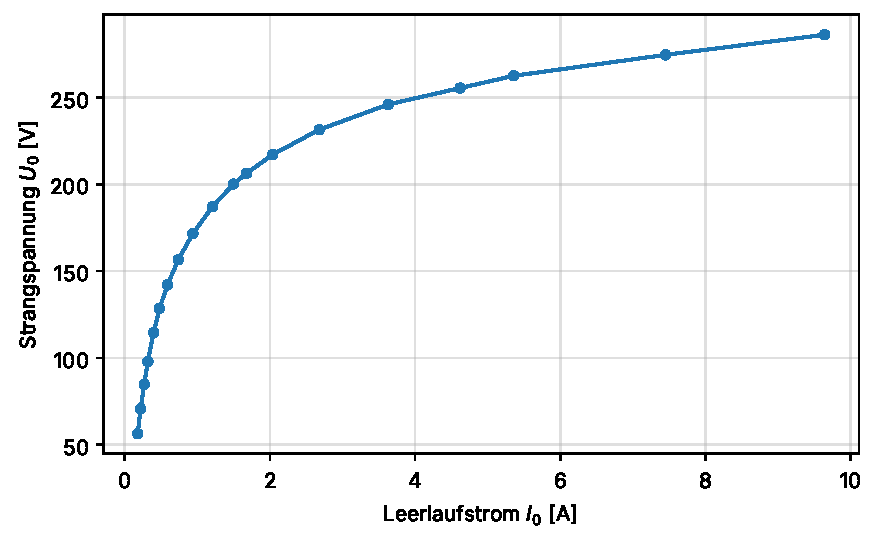
\includegraphics[width=0.85\textwidth]{leerlaufkennlinie.pdf}
\caption{Leerlaufkennlinie $U_0 = f(I_0)$}
\label{fig:ll}
\end{figure}

\Cref{fig:ll} zeigt die typische Magnetisierungskennlinie: Bis etwa \SI{170}{V} steigt der Strom nahezu proportional zur Spannung (linearer Bereich des Eisens). Danach knickt die Kennlinie ab: Der Kern gerät zunehmend in die Sättigung, und der Strom wächst überproportional. Der Nennpunkt liegt bereits im Knie der Kennlinie. Eine Spannungserhöhung um \SI{30}{\percent} auf \SI{286}{V} vergrößert den Leerlaufstrom um den Faktor 4,4 auf \SI{9.6}{A}.

\begin{figure}[H]
\centering
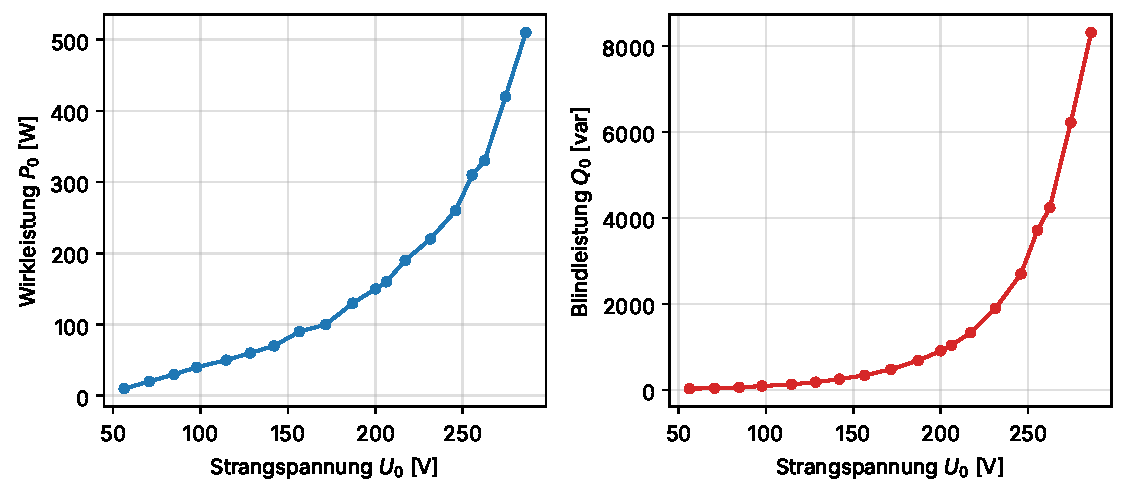
\includegraphics[width=0.85\textwidth]{leerlaufleistung.pdf}
\caption{Leerlaufversuch: Wirkleistung $P_0$ (links) und Blindleistung $Q_0$ (rechts) über der Strangspannung}
\label{fig:llp}
\end{figure}

Die Wirkleistung $P_0$ entspricht den Eisenverlusten (Hysterese- und Wirbelstromverluste). Sie steigt etwa quadratisch mit der Spannung (\cref{fig:llp}, links). Die Blindleistung $Q_0$ (\cref{fig:llp}, rechts) steigt dagegen oberhalb der Nennspannung stark an, da der Magnetisierungsbedarf in der Sättigung explodiert. Entsprechend sinkt der Leistungsfaktor von 0,41 auf 0,06.

Durch lineare Interpolation bei $U_\mathrm{N,Str}=\SI{220}{V}$ ergeben sich die Kennwerte in \cref{tab:ll}. Die Querelemente des Ersatzschaltbilds folgen aus
\begin{equation}
  R_\mathrm{Fe} = \frac{U_\mathrm{N,Str}^2}{P_0/3}, \qquad
  X_\mathrm{h} = \frac{U_\mathrm{N,Str}^2}{Q_0/3}.
\end{equation}

\begin{table}[H]
\centering
\caption{Kennwerte aus dem Leerlaufversuch bei Nennspannung $U_\mathrm{N,Str} = \SI{220}{V}$}
\label{tab:ll}
\begin{tabular}{@{}lr@{}}
\toprule
Größe & Wert\\
\midrule
Leerlaufstrom $I_0$ & \SI{2.17}{A} ($\SI{4.8}{\percent}$ von $I_\mathrm{N}$)\\
Eisenverluste $P_0 \approx P_\mathrm{Fe}$ & \SI{196}{W} ($\SI{0.65}{\percent}$ von $S_\mathrm{N}$)\\
Magnetisierungsblindleistung $Q_0$ & \SI{1445}{var}\\
Leistungsfaktor $\cos\varphi_0$ & 0,13\\
Eisenverlustwiderstand $R_\mathrm{Fe}$ (je Strang) & \SI{741}{\ohm}\\
Hauptreaktanz $X_\mathrm{h}$ (je Strang) & \SI{100.5}{\ohm} ($L_\mathrm{h}\approx\SI{0.32}{H}$)\\
\bottomrule
\end{tabular}
\end{table}

Der Leerlaufstrom ist mit unter \SI{5}{\percent} des Nennstroms klein und nahezu rein induktiv ($\cos\varphi_0 = 0{,}13$). Die Hauptreaktanz ist rund siebenmal kleiner als $R_\mathrm{Fe}$; der Leerlaufstrom besteht also überwiegend aus Magnetisierungsstrom.

%--------------------------------------------------
\section{Kurzschlussversuch}

Die Sekundärklemmen wurden kurzgeschlossen und die Primärspannung vom Stelltransformator aus null langsam erhöht, bis etwa der Nennstrom erreicht war. Gemessen wurde für die Schaltung Yy (Halbstränge in Reihe) und für die Schaltung Yz (Zickzack). Vor dem Kurzschließen wurde bei kleiner Spannung jeweils das Übersetzungsverhältnis bestimmt (\cref{tab:ue}).

\begin{table}[H]
\centering
\caption{Gemessene Übersetzung (Strangspannungen) vor dem Kurzschlussversuch}
\label{tab:ue}
\begin{tabular}{@{}lcccc@{}}
\toprule
Schaltung & $U_{1,\mathrm{Str}}$ / V & $U_{2,\mathrm{Str}}$ / V & $\ue$ gemessen & $\ue$ theoretisch\\
\midrule
Yy & 18,5 & 18,5 & 1,000 & 1\\
Yz & 14,8 & 12,6 & 1,175 & $2/\sqrt3 = 1{,}155$\\
\bottomrule
\end{tabular}
\end{table}

Für Yy stimmt die Übersetzung exakt. Für Yz bestätigt sie die geometrische Addition der Halbstrangspannungen aus \cref{sec:a2}; die Abweichung von \SI{1.7}{\percent} entspricht bei \SI{12.6}{V} und einer Ableseauflösung von \SI{0.1}{V} nur etwa zwei Digits.

Da die Spannung im Kurzschlussversuch klein ist (\SIrange{6}{15}{V} statt \SI{220}{V}), ist der Fluss gering und die Eisenverluste sind vernachlässigbar. Die gemessene Wirkleistung entspricht damit den Kupferverlusten. Die Längselemente ergeben sich je Strang zu
\begin{equation}
  R_\mathrm{k} = \frac{P_\mathrm{k}}{3 I_\mathrm{k}^2}, \qquad
  X_\mathrm{k} = \frac{Q_\mathrm{k}}{3 I_\mathrm{k}^2}, \qquad
  Z_\mathrm{k} = \sqrt{R_\mathrm{k}^2 + X_\mathrm{k}^2}.
\end{equation}
Für jede Schaltung wurde über alle Messpunkte ein Ausgleich (Methode der kleinsten Quadrate) gebildet. Die Kurzschlussspannung bei Bemessungsstrom ist
\begin{equation}
  u_\mathrm{k} = \frac{Z_\mathrm{k}\, I_\mathrm{1N}}{U_\mathrm{N,Str}}, \qquad u_\mathrm{R} = \frac{R_\mathrm{k}\, I_\mathrm{1N}}{U_\mathrm{N,Str}}, \qquad u_\mathrm{X} = \frac{X_\mathrm{k}\, I_\mathrm{1N}}{U_\mathrm{N,Str}}.
\end{equation}
Als primärer Bemessungsstrom gilt bei Yy $I_\mathrm{1N}=\SI{45.5}{A}$ und bei Yz $I_\mathrm{1N}=\SI{39.4}{A}$ (die Sekundärseite begrenzt, siehe \cref{sec:a2}).

\begin{figure}[H]
\centering
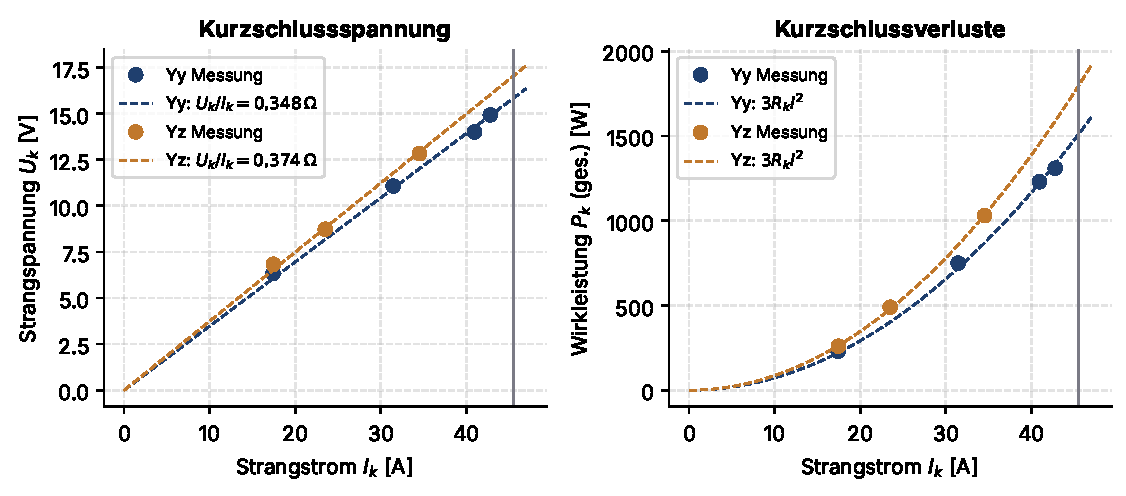
\includegraphics[width=\textwidth]{kurzschluss.pdf}
\caption{Kurzschlussversuch: Strangspannung (links) und Wirkleistung (rechts) über dem Strangstrom}
\label{fig:ks}
\end{figure}

\begin{table}[H]
\centering
\caption{Messwerte und Einzelauswertung des Kurzschlussversuchs (je Strang)}
\label{tab:ks}
\begin{tabular}{@{}lrrrrrr@{}}
\toprule
Schaltung & $U_\mathrm{k}$ / V & $I_\mathrm{k}$ / A & $P_\mathrm{k}$ / W & $Q_\mathrm{k}$ / var & $R_\mathrm{k}$ / \si{\ohm} & $X_\mathrm{k}$ / \si{\ohm}\\
\midrule
Yy & 6,33 & 17,41 & 230 & 250 & 0,253 & 0,275\\
Yy & 11,07 & 31,45 & 750 & 810 & 0,253 & 0,273\\
Yy & 14,93 & 42,80 & 1310 & 1450 & 0,238 & 0,264\\
Yy & 14,00 & 40,96 & 1230 & 1430 & 0,244 & 0,284\\
\midrule
Yz & 6,83 & 17,45 & 260 & 250 & 0,285 & 0,274\\
Yz & 8,73 & 23,50 & 490 & 480 & 0,296 & 0,290\\
Yz & 12,83 & 34,54 & 1030 & 1070 & 0,288 & 0,299\\
\bottomrule
\end{tabular}
\end{table}

\begin{table}[H]
\centering
\caption{Ergebnisse des Kurzschlussversuchs (Ausgleich über alle Messpunkte)}
\label{tab:ks2}
\begin{tabular}{@{}lcc@{}}
\toprule
Größe & Yy & Yz\\
\midrule
Bezugsstrom $I_\mathrm{1N}$ & \SI{45.5}{A} & \SI{39.4}{A}\\
$R_\mathrm{k}$ / $X_\mathrm{k}$ / $Z_\mathrm{k}$ je Strang & 0,243 / 0,273 / \SI{0.366}{\ohm} & 0,289 / 0,296 / \SI{0.414}{\ohm}\\
$\cos\varphi_\mathrm{k}$ & 0,66 & 0,70\\
Kurzschlussspannung $U_\mathrm{k}$ (Strang) & \SI{16.6}{V} & \SI{16.3}{V}\\
rel.\ Kurzschlussspannung $u_\mathrm{k}$ & \SI{7.6}{\percent} & \SI{7.4}{\percent}\\
$u_\mathrm{R}$ / $u_\mathrm{X}$ & \SI{5.0}{\percent} / \SI{5.6}{\percent} & \SI{5.2}{\percent} / \SI{5.3}{\percent}\\
Kupferverluste bei Nennstrom $P_\mathrm{kN}$ & \SI{1508}{W} & \SI{1346}{W}\\
\bottomrule
\end{tabular}
\end{table}

Die Spannung und die Verluste folgen den erwarteten Gesetzmäßigkeiten $U_\mathrm{k}\sim I_\mathrm{k}$ und $P_\mathrm{k}\sim I_\mathrm{k}^2$ (\cref{fig:ks}). Die Impedanz ist damit stromunabhängig, wie es für die eisenlose Streuflussstrecke zu erwarten ist.

Die Zickzackschaltung hat größere Längswiderstände als Yy: $R_\mathrm{k}$ ist etwa \SI{19}{\percent} größer. Der Grund ist, dass sich die Halbstrangspannungen bei Zickzack geometrisch addieren. Für dieselbe Sekundärspannung ist also mehr Wicklungskupfer nötig, das vom vollen Strom durchflossen wird. Auch die Streureaktanz steigt, weil die beiden Halbstränge einer Phase auf verschiedenen Schenkeln liegen und schlechter magnetisch gekoppelt sind.

\begin{hinweis}[Hinweis zur Auswertung]
Bei Yz ist $3\,U_\mathrm{k}I_\mathrm{k}$ etwa \SI{13}{\percent} kleiner als die vom Messgerät angezeigte Scheinleistung $S_\mathrm{k}$. Die drei Stränge sind bei der Zickzackschaltung also nicht exakt symmetrisch belastet, und der angezeigte Mittelwert der Strangspannung beschreibt den Transformator nur ungenau. Die Auswertung nutzt deshalb die über alle drei Stränge summierten Leistungen $P_\mathrm{k}$ und $Q_\mathrm{k}$. Aus $U_\mathrm{k}/I_\mathrm{k}$ allein ergäbe sich $Z_\mathrm{k}\approx\SI{0.35}{\ohm}$ (Yy) bzw.\ \SI{0.37}{\ohm} (Yz) und damit $u_\mathrm{k}\approx\SI{7.2}{\percent}$ bzw.\ \SI{6.7}{\percent}.
\end{hinweis}

%--------------------------------------------------
\section{Belastungsversuch}

Im Belastungsversuch war der Transformator in Yz geschaltet (erkennbar an $U_1/U_2 \approx 1{,}17$). Er wurde mit drei verschiedenen Lasten bei etwa einem Drittel der Bemessungsleistung betrieben. \Cref{tab:bel} zeigt die Messwerte beider Seiten.

\begin{table}[H]
\centering
\small
\setlength{\tabcolsep}{4pt}
\caption{Messwerte des Belastungsversuchs (Strangwerte, Leistungen gesamt)}
\label{tab:bel}
\begin{tabular}{@{}llrrrrrr@{}}
\toprule
Lastfall & Seite & $U$ / V & $I$ / A & $P$ / kW & $Q$ / kvar & $S$ / kVA & $\cos\varphi$\\
\midrule
ohmsch & primär & 221,60 & 15,87 & 10,40 & 1,81 & 10,58 & 0,99\\
 & sekundär & 187,97 & 17,86 & 10,07 & 0,00 & 10,08 & 1,00\\
\midrule
ohmsch-induktiv & primär & 203,60 & 24,26 & 8,50 & 12,14 & 14,82 & 0,58\\
 & sekundär & 168,63 & 26,52 & 7,93 & 10,83 & 13,42 & 0,59\\
\midrule
ohmsch-kapazitiv & primär & 220,57 & 16,04 & 10,09 & 3,30 & 10,62 & 0,95\\
 & sekundär & 188,87 & 19,09 & 9,69 & 4,83 & 10,82 & 0,90\\
\bottomrule
\end{tabular}
\end{table}

\paragraph{Wirkungsgrad und Verluste.} Der Wirkungsgrad folgt direkt aus der Leistungsbilanz:
\begin{equation}
  \eta = \frac{P_2}{P_1}, \qquad P_\mathrm{V} = P_1 - P_2 \approx P_\mathrm{Fe} + P_\mathrm{Cu}.
\end{equation}

\begin{figure}[H]
\centering
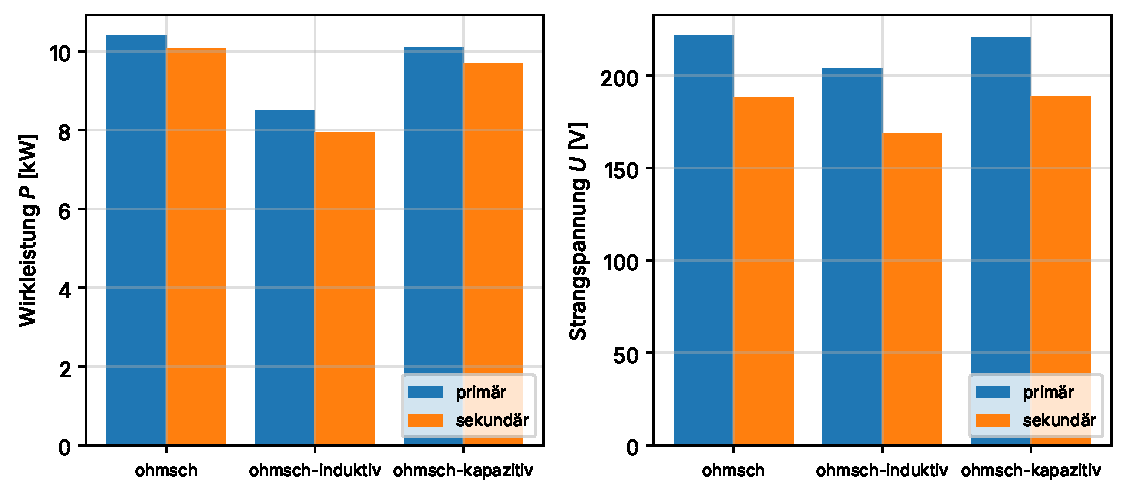
\includegraphics[width=\textwidth]{belastung.pdf}
\caption{Belastungsversuch: Wirkleistung (links) und Strangspannung (rechts) auf Primär- und Sekundärseite}
\label{fig:bel}
\end{figure}

\begin{table}[H]
\centering
\caption{Auswertung des Belastungsversuchs. Erwartete Verluste: $P_\mathrm{Fe}$ aus dem Leerlaufversuch bei $U_1$, $P_\mathrm{Cu}=3R_\mathrm{k}I_1^2$ mit $R_\mathrm{k}$ (Yz)}
\label{tab:bel2}
\begin{tabular}{@{}lccc@{}}
\toprule
Größe & ohmsch & ohmsch-induktiv & ohmsch-kapazitiv\\
\midrule
Wirkungsgrad $\eta$ & \SI{96.8}{\percent} & \SI{93.3}{\percent} & \SI{96.0}{\percent}\\
gemessene Verluste $P_1-P_2$ & \SI{330}{W} & \SI{570}{W} & \SI{400}{W}\\
erwartet $P_\mathrm{Fe}+P_\mathrm{Cu}$ & $199+218=\SI{418}{W}$ & $156+510=\SI{666}{W}$ & $197+223=\SI{420}{W}$\\
\midrule
$U_{20} = U_1/\ue$ ($\ue = 2/\sqrt3$) & \SI{191.9}{V} & \SI{176.3}{V} & \SI{191.0}{V}\\
Spannungsänderung $\Delta u$ gemessen & \SI{2.1}{\percent} & \SI{4.4}{\percent} & \SI{1.1}{\percent}\\
$\Delta u$ nach Kapp & \SI{2.1}{\percent} & \SI{4.9}{\percent} & \SI{1.0}{\percent}\\
\midrule
Blindleistung Trafo $Q_1 - Q_2$ & \SI{1.81}{kvar} & \SI{1.31}{kvar} & \SI{1.53}{kvar}$^{*}$\\
\bottomrule
\end{tabular}\\[0.3em]
{\footnotesize $^{*}$ Primär- und Sekundärseite sind hier kapazitiv; daher $Q_\mathrm{T} = |Q_2| - |Q_1|$.}
\end{table}

Der Wirkungsgrad liegt zwischen \SI{93}{\percent} und \SI{97}{\percent}. Bei induktiver Last ist er am kleinsten: Für etwa dieselbe Wirkleistung fließt wegen $\cos\varphi = 0{,}59$ ein um rund \SI{50}{\percent} größerer Strom, und die Kupferverluste steigen quadratisch. Die gemessenen Verluste liegen jeweils um \SIrange{90}{100}{W} unter dem aus Leerlauf- und Kurzschlussversuch erwarteten Wert. Das ist plausibel, weil $P_1-P_2$ die Differenz zweier großer Zahlen ist: Schon \SI{0.5}{\percent} Messfehler auf jeder Seite ergeben etwa \SI{100}{W}.

\paragraph{Spannungsänderung.} Die relative Spannungsänderung gegenüber dem Leerlauf
\begin{equation}
  \Delta u = \frac{U_{20} - U_2}{U_{20}}, \qquad
  \Delta u_\mathrm{Kapp} \approx \frac{I_1\,(R_\mathrm{k}\cos\varphi_2 + X_\mathrm{k}\sin\varphi_2)}{U_1}
\end{equation}
($\sin\varphi_2 < 0$ bei kapazitiver Last) wurde mit der Bemessungsübersetzung $\ue=2/\sqrt3$ berechnet. Gemessene und nach Kapp berechnete Werte stimmen sehr gut überein (\cref{tab:bel2}). Wird stattdessen die bei kleiner Spannung gemessene Übersetzung $1{,}175$ verwendet, ergibt sich \SI{0.4}{\percent}, \SI{2.7}{\percent} bzw.\ \SI{-0.6}{\percent}. Die Bemessungsübersetzung ist also die bessere Bezugsgröße; der Wert 1,175 ist durch die Ableseauflösung verfälscht.

Die induktive Last verursacht den größten Spannungsfall, weil $X_\mathrm{k}\sin\varphi_2$ und $R_\mathrm{k}\cos\varphi_2$ sich addieren. Bei kapazitiver Last wirkt $X_\mathrm{k}\sin\varphi_2$ dem ohmschen Anteil entgegen, und der Spannungsfall ist am kleinsten. Bei stärker kapazitiver Last kann die Sekundärspannung sogar über die Leerlaufspannung steigen (Ferranti-ähnlicher Effekt). Zusätzlich brach bei induktiver Last die Netzspannung von \SI{221}{V} auf \SI{204}{V} ein, weil der hohe Blindstrom auch an der Netz- und Stelltrafoimpedanz Spannung abfallen lässt.

\paragraph{Blindleistungsbedarf.} Der Transformator selbst nimmt induktive Blindleistung auf: im Querzweig $Q_0 \approx \SI{1.45}{kvar}$ und im Längszweig $3X_\mathrm{k}I^2 \approx \SIrange{0.2}{0.5}{kvar}$. Die Differenzen $Q_1-Q_2$ von \SIrange{1.3}{1.8}{kvar} bestätigen das. Bei kapazitiver Last kompensiert der Transformator einen Teil der kapazitiven Blindleistung, daher ist $|Q_1| < |Q_2|$. Auch das Stromverhältnis $I_2/I_1 = 1{,}09$ bis $1{,}19$ weicht vom idealen $\ue=1{,}155$ ab, weil sich der Magnetisierungsstrom zum umgerechneten Laststrom geometrisch addiert.

%--------------------------------------------------
\section{Einschaltstrom (Rush-Effekt)}

Der leerlaufende Transformator wurde dreimal direkt ans Netz ($U_\mathrm{Str}\approx\SI{213}{V}$) geschaltet. Das Oszilloskop wurde auf den Strom getriggert (Triggerschwelle \SI{-36.3}{A}). \Cref{fig:rush} zeigt die aufgezeichneten Verläufe, \cref{fig:scope} beispielhaft ein Oszilloskopbild.

\begin{figure}[H]
\centering
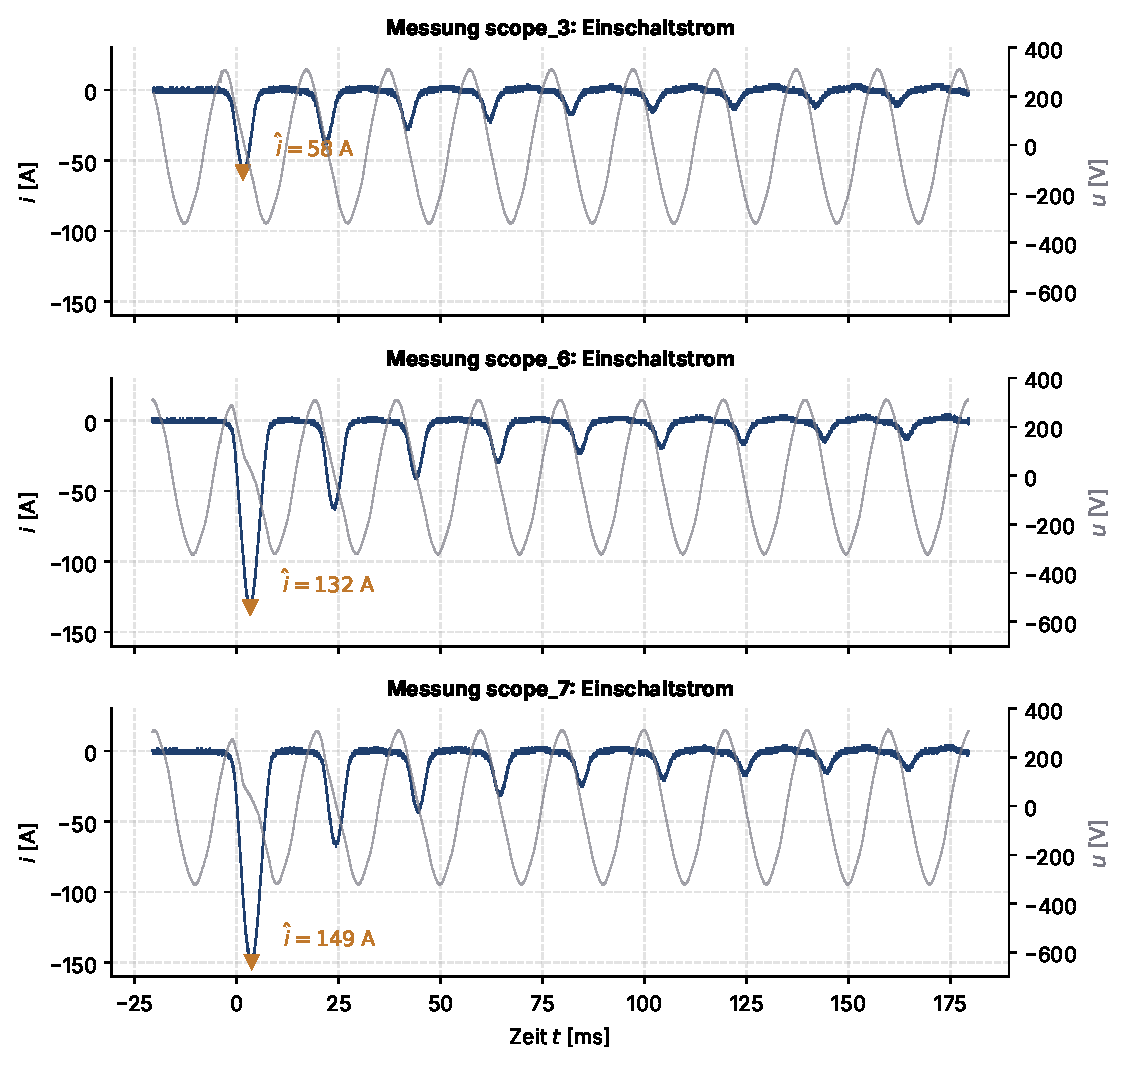
\includegraphics[width=0.95\textwidth]{rush.pdf}
\caption{Einschaltstrom $i_1(t)$ (blau, linke Achse) und Strangspannung $u_1(t)$ (rot, rechte Achse) für drei Einschaltvorgänge}
\label{fig:rush}
\end{figure}

\begin{figure}[H]
\centering
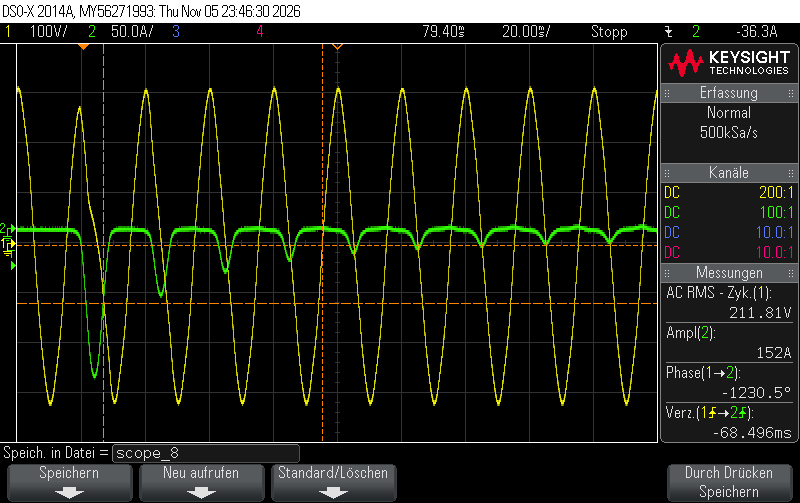
\includegraphics[width=0.75\textwidth]{scope_8.png}
\caption{Oszilloskopbild eines Einschaltvorgangs (gelb: Spannung, \SI{100}{V/div}; grün: Strom, \SI{50}{A/div}; \SI{20}{ms/div})}
\label{fig:scope}
\end{figure}

\begin{table}[H]
\centering
\caption{Scheitelwerte des Einschaltstroms je Netzperiode}
\label{tab:rush}
\begin{tabular}{@{}lrrrrrrrrr@{}}
\toprule
Periode & 1 & 2 & 3 & 4 & 5 & 6 & 7 & 8 & 9\\
\midrule
Messung 1 (scope\_3) / A & 58 & 38 & 28 & 23 & 18 & 16 & 14 & 13 & 12\\
Messung 2 (scope\_6) / A & 132 & 63 & 41 & 30 & 24 & 20 & 17 & 16 & 14\\
Messung 3 (scope\_7) / A & 149 & 68 & 44 & 32 & 25 & 21 & 18 & 16 & 14\\
\bottomrule
\end{tabular}
\end{table}

Die Messungen zeigen alle Merkmale des Rush-Effekts aus \cref{sec:a4}:
\begin{itemize}[nosep]
  \item \textbf{Hohe Stromspitzen:} Der Scheitelwert erreicht bis zu \SI{149}{A}. Das ist das 2,3-fache des Nennstrom-Scheitelwerts ($\sqrt2\cdot\SI{45.5}{A}=\SI{64}{A}$) und etwa das 50-fache des Leerlaufstrom-Scheitelwerts ($\sqrt2\cdot\SI{2.17}{A}=\SI{3.1}{A}$).
  \item \textbf{Einseitige Stromimpulse:} Der Strom fließt nur in einer Richtung (negativ). Ursache ist der Gleichanteil des Flusses, der den Kern nur in einer Halbwelle in die Sättigung treibt.
  \item \textbf{Lage der Spitzen:} Die Maxima liegen jeweils im Nulldurchgang der Spannung ($u\approx\SI{25}{V}$). Dort ist der Fluss $\Phi = \frac{1}{N}\int u\,\mathrm{d}t$ maximal und damit die Sättigung am stärksten.
  \item \textbf{Abklingen:} Der Gleichanteil wird über die Wicklungswiderstände abgebaut. Die Spitze halbiert sich zunächst von Periode zu Periode und klingt dann langsamer ab. Nach neun Perioden (\SI{180}{ms}) fließen noch etwa \SI{14}{A}, also weiterhin ein Vielfaches des stationären Leerlaufstroms.
  \item \textbf{Streuung:} Die drei Spitzenwerte unterscheiden sich stark (58, 132 und \SI{149}{A}), obwohl der Versuch gleich durchgeführt wurde. Der Einschaltzeitpunkt (Phasenwinkel) und die Remanenz des Kerns sind zufällig und bestimmen, wie weit der Fluss in die Sättigung getrieben wird.
\end{itemize}

%==================================================
\chapter{Fazit}

Im Versuch wurden die Kennwerte und das Betriebsverhalten eines \SI{30}{kVA}-Drehstromtransformators messtechnisch bestimmt. Die Ergebnisse bestätigen das Ersatzschaltbild und die Theorie aus der Vorbereitung weitgehend.

\section{Zusammenfassung der Ergebnisse}

\begin{table}[H]
\centering
\caption{Übersicht der ermittelten Kennwerte}
\label{tab:fazit}
\begin{tabular}{@{}ll@{}}
\toprule
Größe & Ergebnis\\
\midrule
Leerlaufstrom $I_0$ bei \SI{220}{V} & \SI{2.17}{A} (\SI{4.8}{\percent} $I_\mathrm{N}$)\\
Eisenverluste $P_\mathrm{Fe}$ bei \SI{220}{V} & \SI{196}{W} (\SI{0.65}{\percent} $S_\mathrm{N}$)\\
$R_\mathrm{Fe}$ / $X_\mathrm{h}$ je Strang & \SI{741}{\ohm} / \SI{100.5}{\ohm}\\
$R_\mathrm{k}$ / $X_\mathrm{k}$ je Strang (Yy) & \SI{0.243}{\ohm} / \SI{0.273}{\ohm}\\
$R_\mathrm{k}$ / $X_\mathrm{k}$ je Strang (Yz) & \SI{0.289}{\ohm} / \SI{0.296}{\ohm}\\
Kurzschlussspannung $u_\mathrm{k}$ (Yy / Yz) & \SI{7.6}{\percent} / \SI{7.4}{\percent}\\
Kupferverluste bei Nennstrom (Yy / Yz) & \SI{1.51}{kW} / \SI{1.35}{kW}\\
Übersetzung Yy / Yz & 1,000 / 1,175 (theor.\ 1 / 1,155)\\
Wirkungsgrad ohmsch / induktiv / kapazitiv & \SI{96.8}{\percent} / \SI{93.3}{\percent} / \SI{96.0}{\percent}\\
Spannungsänderung ohmsch / induktiv / kapazitiv & \SI{2.1}{\percent} / \SI{4.4}{\percent} / \SI{1.1}{\percent}\\
max.\ Einschaltstrom (Scheitel) & \SI{58}{A} bis \SI{149}{A} ($\le 2{,}3\cdot\hat\imath_\mathrm{N}$)\\
\bottomrule
\end{tabular}
\end{table}

\section{Schlussfolgerungen}

\begin{enumerate}
  \item \textbf{Leerlauf:} Der Transformator arbeitet bei Nennspannung im Knie der Magnetisierungskennlinie. Das nutzt das Eisen gut aus, macht ihn aber empfindlich gegen Überspannung: Bei \SI{130}{\percent} Spannung steigt der Leerlaufstrom auf das 4,4-fache. Die Eisenverluste sind mit \SI{0.65}{\percent} der Bemessungsleistung klein und fallen unabhängig von der Last ständig an.
  \item \textbf{Kurzschluss:} Mit $u_\mathrm{k}\approx\SI{7.5}{\percent}$ liegt der Transformator im typischen Bereich für Verteiltransformatoren dieser Größe. Ein satter Kurzschluss an Nennspannung würde den $1/u_\mathrm{k}\approx 13$-fachen Nennstrom treiben. Die Kupferverluste bei Nennstrom sind fast achtmal größer als die Eisenverluste.
  \item \textbf{Schaltungsvergleich:} Die Zickzackschaltung hat höhere Längswiderstände und nutzt die Wicklung nur zu \SI{86.6}{\percent} aus. Sie wird trotzdem eingesetzt, weil sie unsymmetrische Lasten (Sternpunktbelastung) gut verträgt.
  \item \textbf{Belastung:} Wirkungsgrad und Spannungshaltung hängen stark vom Leistungsfaktor ab. Induktive Lasten verursachen den größten Spannungsfall und die größten Verluste; kapazitive Lasten heben die Spannung an. Das Ersatzschaltbild aus Leerlauf- und Kurzschlussversuch sagt den Spannungsfall (Kapp) sehr genau voraus.
  \item \textbf{Wirkungsgradmaximum:} Das Maximum liegt dort, wo die Kupferverluste gleich den Eisenverlusten sind, also bei $I/I_\mathrm{N}=\sqrt{P_\mathrm{Fe}/P_\mathrm{kN}}\approx\sqrt{196/1508}\approx 0{,}36$. Die ohmsche Messung lag mit etwa einem Drittel der Bemessungsleistung nahe an diesem Punkt.
  \item \textbf{Rush-Effekt:} Der Einschaltstrom kann trotz kleinem Leerlaufstrom den Nennstrom deutlich übersteigen und streut stark. Schutzeinrichtungen müssen ihn tolerieren, z.\,B.\ über träge Sicherungen oder eine Sperrung anhand der 2.~Harmonischen, ohne beim echten Fehler zu versagen. Gegenmaßnahmen sind in \cref{sec:a4} beschrieben.
\end{enumerate}

\section{Fehlerbetrachtung}

\begin{itemize}
  \item \textbf{Auflösung der Leistungsmessgeräte:} Wirk- und Blindleistungen werden mit \SI{10}{W} bzw.\ \SI{10}{var} Auflösung angezeigt. Im Leerlauf bei kleinen Spannungen (z.\,B.\ $P_0=\SI{10}{W}$) ist der relative Fehler daher groß; das betrifft besonders den Leistungsfaktor.
  \item \textbf{Differenzbildung:} Die Verluste im Belastungsversuch sind die Differenz zweier großer Leistungen. Ein Fehler von \SI{0.5}{\percent} pro Messgerät verursacht bereits $\approx\SI{100}{W}$ Abweichung. Das erklärt die Differenz zur Vorhersage.
  \item \textbf{Übersetzung bei kleiner Spannung:} Die Messung bei etwa \SI{15}{V} mit \SI{0.1}{V} Auflösung ergibt für Yz 1,175 statt 1,155. Die Bemessungsübersetzung beschreibt das Verhalten unter Last besser.
  \item \textbf{Unsymmetrie bei Yz:} Die Strangspannungsanzeige weicht bei Zickzack um rund \SI{13}{\percent} von $S/(3I)$ ab; die strangweise Auswertung ist deshalb unsicherer als bei Yy.
  \item \textbf{Erwärmung:} Bei Kurzschluss- und Belastungsversuch erwärmen sich die Wicklungen. $R_\mathrm{k}$ steigt dadurch (Kupfer: $\approx\SI{0.4}{\percent/K}$). Die Temperatur wurde nicht protokolliert; die Streuung der Einzelwerte ($R_\mathrm{k}=\SIrange{0.238}{0.253}{\ohm}$ bei Yy) liegt im Bereich der Ablesegenauigkeit.
  \item \textbf{Netzspannung:} Die Netzspannung schwankte (\SI{204}{V} bis \SI{222}{V}). Im Belastungsversuch waren die Arbeitspunkte deshalb nicht exakt vergleichbar.
  \item \textbf{Oszilloskop:} Die Stromzange (100:1) quantisiert in Stufen von etwa \SI{0.5}{A}. Das ist für die Spitzenwerte (\SIrange{58}{149}{A}) unerheblich, verrauscht aber den Ruhestrom.
\end{itemize}

Insgesamt wurden alle Versuchsziele erreicht. Der Versuch zeigt anschaulich, wie sich aus zwei einfachen Messungen (Leerlauf und Kurzschluss) ein Ersatzschaltbild ableiten lässt, das das Betriebsverhalten unter Last zuverlässig vorhersagt.

%==================================================
\bibliography{Literatur}
\end{document}
